
\chapter[Motivations and Precursors of RPHash]{Motivations and Precursors of RPHash}
\chaptermark{Pre-RPHash}
\label{motive}

In this chapter we will describe the motivations behind the \textsf{RPHash} algorithm, and give an overview of the \textsf{RPHash}
algorithm's goals.  The general idea of \textsf{RPHash} is motivated by a particularly degenerate case of the LSH-based $k$
nearest neighbors ($k$NN) problem known as $cr$-NN.  Briefly, the nearest neighbor problem is the problem of finding the
closest analog in a database to an unknown data vector.

\section{Bad $k$NN}
In one-dimension, the NN problem is solvable in log-time via a binary search of the dataset.  Similarly, in
two-dimensions it is also solvable in log-time via the point location algorithm over the Voronoi partitioned dataset.
The log bound unfortunately fails as dimensionality grows greater than 2, mainly due to the exponential growth of the
Voronoi region set $n^{\theta(d)}$.  Data structures such as k-d Trees\cite{Bentley-75} can be constructed to provide log-time average search
complexity for uniform datasets up to about 32 dimensions ($N >> 2^d$, $N=$ size of Database).  Beyond that however, k-d tree
search tends to degenerate into the linear scan search algorithm.  Naively this problem can be solved by the linear scan
algorithm (shown in Algorithm \ref{linearscan}) which consists of sorting a list of distances between the query vector
and all vectors in the dataset then returning the nearest $k$ vectors.

\begin{Definition}[Nearest Neighbor] \cite{Samet}\\
Given a set of vectors $P$ in $R^d$ and query vector $q$ return $k$ vectors $p\subseteq P$ such that
$p=\text{Argmin}\{dist(p',q)\}$, where dist is some metric function.
\end{Definition}

\begin{algorithm}
\RestyleAlgo{boxruled}
\caption{Linear Scan, Query $q$, dataset $X$\label{linearscan}}
\DontPrintSemicolon
$k$NN$ = X[0:k]$\\
\ForAll{$x \in X[k:n]$} 
{	
      \If{$\lVert x,q\lVert_2 < \lVert q,k$NN$[0]\lVert_2$}
      {
	$k$NN$[0]=x$\\
	$k$NN$ = sort(k$NN$)$\\
      }
}
\textbf{Return:} $k$NN
\end{algorithm}

This algorithm requires that we compute distances between every vector in the dataset and our query vector $\theta{nd}$.
If we could somehow omit vectors that we know are not anywhere near our input vector, we could certainly speed up our
calculation and possibly solve $k$NN in a sub-linear time.  This is the intuition of the LSH-$k$NN algorithm.
Previously discussed LSH functions can be used to winnow the field of candidate near neighbors that need to be searched
via the linear scan method. A considerable amount of computation can be avoided by performing this large volume
reduction on the query dataset provided some error is tolerable.  The basic outline of LSH-based $k$NN is given in
Algorithm \ref{lshnn} and Algorithm \ref{lshnnq}.

\begin{algorithm}
\RestyleAlgo{boxruled}
\caption{Preprocessing on Dataset X \label{lshnn}}
\DontPrintSemicolon
\ForAll{$x \in X$} 
{	id = LSH\_Hash(x)\\
	$T$[id].add$(x)$\\
}
\textbf{Return:} $T$
\end{algorithm}
\begin{algorithm}
\RestyleAlgo{boxruled}
\caption{Query $k$ nearest to $q$ in X, using hashtable $T$\label{lshnnq}}
\DontPrintSemicolon
id = LSH\_Hash($q$)\\
\textbf{Return:} linear\_scan($T$[id],$k$)\\
\end{algorithm}

Assuming the LSH\_Hash function is sufficiently discriminative, an appropriately chosen locality sensitive hash
functions can achieve a complexity bound of $\theta(n^\rho+log(n))$ where $\rho$ is determined by the selectivity of the
hash function.  LSH-$k$NN is a highly successful solution to the nearest neighbor problem in high dimensions.  However,
a degenerate case of the LSH-$k$NN structure occurs when the candidate field becomes quite large.  These degenerate
cases represent an outlier condition for $cr$-NN algorithm, and often contributes to the algorithm's worse-case
performance.  While this outlier example presents a problem to $cr$-NN, viewed under a different problem requirement, it
becomes beneficial for quickly identifying candidate density modes.

In Figure \ref{lshclust} we give give a toy example of the basic concept for or proposed Random Projection Hash algorithm.
The example contains 4 vectors, 3 of are somewhat close to one another in $\mathbb{R}^2$.  The space is randomly bisected along
4 partitioning plains, corresponding to 4 hash functions and 8 regions.  Inspecting the high cardinality hash buckets, we see
they often, but not always, correspond to high density regions.  In this case our small cluster of 3 items. The
correspondence between high cardinality hash buckets and high density partitions, forms the basis of our algorithms.
\begin{figure}
    \centerline{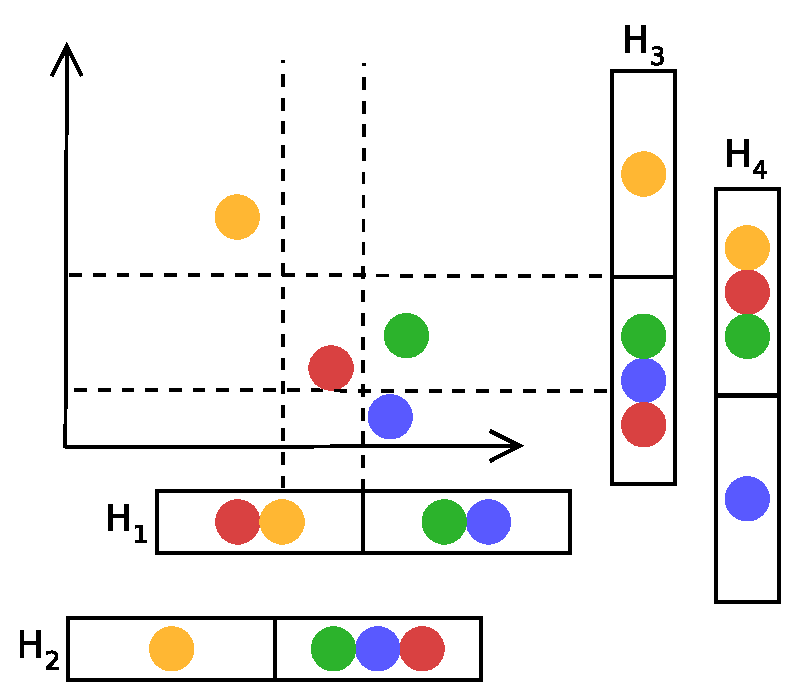
\includegraphics[width=.6\textwidth]{figs/multiLSHClustering}}
    \caption{Example of an orthogonal LSH on $\mathbb{R}^2$ Data}\label{lshclust}
\end{figure}

\section{Cardinality Shift Clustering}
Previous work on graphics processing unit (GPU) accelerated $cr$-NN \cite{carraher} lead to a generous speedup per GPU core for bulk NN search.
One problem that could take advantage of this acceleration to bulk NN search is the LSH accelerated Mean Shift algorithm
of Li \emph{et al} \cite{Li09}.  Although this still remains an interesting use case, a more interesting case was
investigated where the generative nature of decoder functions could be used to optimize interprocess communication in
distributed systems.  In this dissertation, vectors would be assigned to processing nodes using the LSH function, resulting
in better vector locality.  Furthermore this proposed method would use LSH bucket cardinality as a proxy for the
computational and communication inefficient mean shift step shown in Figure \ref{unreferencedFigure}.

\begin{figure}
\[
\overset{\rightarrow}{x}= {{\sum_{x_i\in N_(x)}
{K'({x-x_i})\overset{\rightarrow}{x}}}\over {\sum_{x_i\in N_(x)} {K'({x-x_i)}}
}}
\]
\caption{Mean-Shift Iteration \cite{Li09}}\label{unreferencedFigure}
\end{figure}

This algorithm is referred to as \emph{Cardinality Shift Clustering} (CSC).  The overall iteration of CSC is similar to
the mode finding step in the mean-shift clustering algorithm \cite{comaniciu-02, carreira, meanshift} with a
focus on scalability and low compute node interdependency.  To get better vector-node locality and minimize
communication overhead a two step course-grain and fine-grain shift is considered.

\subsection{Fine-Grain Iteration}

The fine-grain iteration is similar to mean-shift clustering update step except that it occurs on a finite set of
vectors contained within the bounds of a the partition of the well known Leech Lattice.  Due to this lattice's fixed
dimensionality, conversion between vectors of $\mathbb{R}^d$ and $\mathbb{R}^{24}$ must be performed by random
projection and the pseudo-inverse(or $\epsilon$-suitable inverse) of the projection \cite{bingham}.  Furthermore, this
clustering occurs on a per-compute node basis (Figure \ref{csc}, region \textbf{II}) and each compute node is assigned a
subset of lattice regions (Figure \ref{csc}, region \textbf{I}).  The lattice region IDs are generative and can be
assigned either by truncating the ID mod the number of available compute nodes or some other more advanced load
balancing technique.%% based on the number of vectors per compute node.

Using techniques from Andoni \cite{Andoni} and an addition from Carraher \cite{carraher2}, computation of the function
$N(\cdot)$ of near neighbors for a given point can be performed in nearly optimal $\Theta(n^\rho)$-time.  For a Leech
lattice hash function where $d \leq24$, $\rho \approx 0.2671 $ \cite{Andoni}, while linear search requires $\Theta(d
n)$-operations.  This gives an internal clustering complexity of $\Theta(k n^{1+\rho})$ where $k$ is the maximum
neighborhood size.  By adding the random projection aspects to this iteration, it is believed we will achieve some
tempering to the error surface across multiple projections which may help avoid some local minima of the density modes
by smoothing out point discontinuities.  Furthermore, the sigma value for an Gaussian, $N(\mu,\sigma)$ distribution in
the random projection may allow us to control tempering.

\subsection{Course Grain Iteration}

Due to the $\Theta(n^2)$ complexity of mean-shift clustering, we attempt to mitigate vector to vector communication
scalability by replacing it with a lattice-region to lattice-region course communication step.  All lattice-regions
contain a finite set of vectors.  In CSC we use the cardinality of the sets as weighted components for generating the
course-grain shift vectors, again using the standard kernel mean shift algorithm (Figure \ref{csc}, region
\textbf{III}).  The shift vectors are then broadcast to all computing nodes in the system.

\begin{figure}
    \centerline{\includegraphics[width=.8\textwidth]{figs/csc}}
\caption{Cardinality Shift Clustering}{\textbf{I.} Initial lattice assignment, \textbf{II.} Fine Grain Iteration,
  \textbf{III.} Course Grain Iteration, \textbf{IV.} Updated Positions}\label{csc}
\end{figure}

\subsection{Update Step}
Per compute node, the update step consists of updating all vectors current positions by applying the results of the
course-grain mean-shift vectors within a lattice region for a random projection (Figure \ref{csc}, region \textbf{IV}).
After this, we invert our random projection matrix and apply it to all the vectors giving us a set of (number of random
projections) vectors for each vector in our original $\mathbb{R}^d$ space.  We then average the vectors various random
projections to attain an $d$ dimensional representation that is near the actual result of a full mean-shift clustering
iteration for that vector.  Once the representations of the shifted vectors are averaged in $\mathbb{R}^d$, we again
project the vectors down to 24-dimensional space.  The assumption here is that the global shift will have altered the
lattice-regions for vectors near the borders of a region.  The vectors that have new lattice-region assignments first
check the current compute node for the new lattice-region assignment(a mod lattice ID can easily be tested here).  If
they are not contained in the current compute node, the vector must be sent to the compute node containing its new
lattice-region assignment.  The amount of transfer needed is hopefully minimal and point-to-point.

\subsection{Stopping Condition}

The number of lattice-region assignments should naturally decrease as vectors are pulled toward higher density
lattice-regions.  By counting the number of inter-compute node vector communications (the number of vectors whose
lattice-region assignments have changed), we can get an estimate of the overall entropy remaining in the system on a per
step basis.  As with other machine learning algorithms, the entropy will likely decrease with an inverse
power-distribution.  Suitable stopping conditions are well studied and have been defined for distributions based on
derivative and statistical analysis.

While this method may still have some use as a communication optimization technique for more robust clustering
algorithms such as distributed mean-shift and filtration algorithms for topological data analysis, its complexity may be
unneeded.  The first step of CSC alone turns out to be a sufficient process for general data clustering.  We will
describe the setup of this technique in the following section.

\section{Big Bucket Search}

In the initial development of CSC came a simple test application.  In the test application, a test set
$S=\{S_1,...S_c\}$ of clusters where $S_j = \{x_{j,1},...,x_{j,(n/c)}\}$ and $x_{ij}\in \mathbb{R}^{24}$ were generated
from $C$ Gaussian distributions with $\mu=0,\sigma=\frac{1}{\sqrt{24}} $.  The vectors from the $C$ clusters were
processed using the Lookup-DB generation step of Andoni's \cite{Andoni} Leech Lattice based $cr$-NN algorithm. The full
DB was then scanned through to identify the largest $\epsilon C$ buckets, corresponding to a representative hash ID.
For low variance, the largest buckets corresponded directly to the nearest points of the generated centroids.  This
simple test demonstrated a basic principle of the \textsf{RPHash} algorithm: locating low variance Gaussian Centroid.  As shown
in Figure \ref{bbvar} this basic algorithm works for low-variance Gaussian data, some modifications are needed for
clustering real world data.

\begin{figure}
  \centerline{\includegraphics[width=.8\textwidth]{figs/PRvaryClusters}}
  \caption{PR ``Big Bucket'' Count}{Precision Recall For ``Big Bucket'' and Projected K-Means As a Function Inter-Cluster Variance }\label{bbvar}
\end{figure}

In signal data, a similar process making use of windowing and kernel functions to estimate kernel density is the
Parzen's kernel density estimator \cite{parzen-62}.  Kernel density estimation and clustering are related through the similar concepts of
classes and clusters. While clusters are often defined by the data, classes can be defined by a set of constraints,
both of which can be resolved to the other.  Thus, Parzen's offers a solution to clustering, however dynamic programming
solutions such as this are restricted to 1-dimensional data.

Due to our goal of providing a general clustering solution to dimensions beyond what Parzen's is applicable to, we must
extend the kernel windowing method to arbitrary space partitioning.  Immediately, one could apply a metric partitioning
scheme such as $\mathbb{D}_n$ to the data space, and keep track of the largest partitions.  In fact this is the
principle concept behind many density scan based methods.  These methods are efficient for the lower dimensional regimes
but tend to break down as $d$ increases beyond 10-18 dimensions.  This result is similar to the efficiency breakdown of
k-d tree solutions to $k$NN, and is often regarded as an effect of the curse of dimensionality (\emph{COD})--- distance
metric loosing its specificity.  We again adopt another technique from approximate $k$NN, and apply an ensemble of
projections to high dimensional data.
%And like $k$NN solutions to this problem, we shall adopt the LSH solution for thos problem and use sets of LSH
%functions to probabilistically converge on the lower bound of an ensemble of approximate solutions.
These observation along with various modifications, are the basis for the \textsf{RPHash} Algorithm whose description and
analysis constitute the remainder of this work.